\documentclass[10pt, letterpaper]{article}

\usepackage[utf8]{inputenc}
\usepackage[T1]{fontenc}
\usepackage{geometry}
\usepackage{graphicx}
\geometry{margin=1in}
\usepackage{listings} 
\usepackage{xcolor} 
\usepackage{caption} 
\usepackage{hyperref} 
\usepackage{tocloft} 
\usepackage{enumitem} 

\lstset{
    language=C,
    keywordstyle=\color{blue}\bfseries,
    commentstyle=\color{green!60!black},
    basicstyle=\ttfamily\footnotesize,
    breakatwhitespace=false,
    breaklines=true,
    captionpos=b,
    keepspaces=true,
    showspaces=false,
    showstringspaces=false,
    showtabs=false,
    tabsize=4,
    frame=single,
    rulecolor=\color{gray!30},
    xleftmargin=10pt,
    xrightmargin=10pt,
    belowcaptionskip=10pt,
    aboveskip=12pt,
    belowskip=12pt
}

\title{IPv6 \& IoT: \\ Implementation of a Kernel Space Module and User
Space Utility for retrieving L2 Network Interface Information}
\author{Andrii Konotop}
\date{April 2025}

\begin{document}

\maketitle

\tableofcontents
\newpage

\section{Introduction}
The motivation for this project is to establish a flexible and robust inter-process
communication (IPC) between user space and kernel space using Generic Netlink. The
subject of the communication is the retrieval of Layer 2 (L2) network interface
information. This information is obtained in kernel space using an appropriate kernel API.
The project includes a user-space utility that queries and presents the retrieved data in
two formats. The first format displays a comprehensive list of L2 network interfaces,
including basic details such as interface name, Maximum Transmission Unit (MTU), MAC
address, broadcast address, and transmit (TX) queue length. The second format enables
users to query interface-specific statistics, including the number of good bytes received
and transmitted, the total number of received errors, and the number of transmit problems.

\section{Background}
Netlink, introduced in Linux 2.2 (1999), originally provided a fixed set of protocol
families for different kernel subsystems (e.g., routing, firewall, audit). As Netlink's
popularity grew, the limited range of family numbers became a concern. To address this,
the Linux kernel introduced the Generic Netlink family in version 2.6.15 (released in
2006), allowing dynamic allocation of logical families under a single protocol. When user
space requests a family ID, the kernel’s Generic Netlink controller matches the requested
name to a registered family and replies with the dynamically assigned numeric family ID.
This ID is then used for all further communication with that Generic Netlink family.
Moreover, Generic Netlink enforces TLV attribute payloads, and validates messages using
explicit policies, making the API more straightforward and secure.

\section{Implementation Details}

\subsection{Kernel Module}
The kernel module implements a Generic Netlink family to facilitate communication between
kernel space and user space for retrieving Layer 2 (L2) network interface information. Before
registering the family, its name, attributes, nested sub-attributes, and commands must be
defined. These definitions are shared between the kernel module and the user-space utility
to ensure consistent communication.

The Type-Length-Value (TLV) attribute format supports nested sub-attributes, allowing
related attributes to be grouped under a top-level attribute. This structure simplifies
attribute type validation through the \texttt{nla\_policy} structure, which defines
policies for both parent and nested sub-attributes. In this implementation, a single
top-level attribute, \texttt{NL\_UTIL\_A\_NETDEV}, encapsulates several nested
sub-attributes, including \texttt{NL\_UTIL\_NESTED\_A\_IFINDEX},
\texttt{NL\_UTIL\_NESTED\_A\_IFNAME}, \texttt{NL\_UTIL\_NESTED\_A\_IFMTU}, and others,
corresponding to L2 interface information being transmitted.

\begin{lstlisting}[caption={Top-level and nested attribute definitions}]
enum NL_UTIL_ATTRS {
    NL_UTIL_A_UNSPEC,      /* Unspecified attribute (placeholder) */
    NL_UTIL_A_NETDEV,      /* Network interface-related attribute */
    __NL_UTIL_A_MAX        /* Internal max value for validation */
};
enum NL_UTIL_NESTED_ATTRS {
    NL_UTIL_NESTED_A_UNSPEC,    /* Unspecified nested sub-attribute (placeholder) */
    NL_UTIL_NESTED_A_IFINDEX,   /* Interface index (e.g., 2 for eth0) */
    NL_UTIL_NESTED_A_IFNAME,    /* Interface name (e.g., "eth0") */
    NL_UTIL_NESTED_A_IFMTU,     /* Interface MTU (maximum transmission unit) */
    __NL_UTIL_NESTED_A_MAX      /* Internal max value for validation */
};
\end{lstlisting}

The Generic Netlink family relies on commands and their corresponding callback functions,
registered via the \texttt{genl\_ops} structure during initialization. Two commands are
defined: \texttt{NL\_UTIL\_C\_L2\_LIST} and \texttt{NL\_UTIL\_C\_L2\_IID}.

\begin{lstlisting}[caption={Commands}]
enum NL_UTIL_CMDS {
    NL_UTIL_C_UNSPEC,               /* Unspecified command (placeholder) */
    NL_UTIL_C_L2_LIST,              /* List all Layer 2 network interfaces */
    NL_UTIL_C_L2_IID,               /* Query a Layer 2 interface by index */
    __NL_UTIL_C_MAX                 /* Internal max value for validation */
};
\end{lstlisting}

The \texttt{NL\_UTIL\_C\_L2\_LIST} command is associated with the \texttt{l2\_list\_doit}
callback function. And the \texttt{NL\_UTIL\_C\_L2\_IID} command is associated with the
\texttt{l2\_iid\_doit} callback function.

\begin{lstlisting}[caption={Callback function signatures}]
int l2_list_doit(struct sk_buff *sender_buff, struct genl_info *info);
int l2_iid_doit(struct sk_buff *sender_buff, struct genl_info *info);
\end{lstlisting}

\begin{lstlisting}[caption={Operations}]
struct genl_ops nl_util_gnl_ops[NL_UTIL_C_MAX] = {
    {
        .cmd = NL_UTIL_C_L2_LIST,       /* Command to list L2 interfaces */
        .doit = l2_list_doit,           /* Callback handler for listing interfaces */
    },
    {
        .cmd = NL_UTIL_C_L2_IID,        /* Command to get interface by index */
        .doit = l2_iid_doit,            /* Callback handler for interface lookup */
    },
};
\end{lstlisting}

The \texttt{NL\_UTIL\_C\_L2\_IID} command expects an additional interface index as a part
of payload. The \texttt{l2\_iid\_doit} callback parses this index from the nested
sub-attribute structure (\texttt{NL\_UTIL\_A\_NETDEV} $\rightarrow$
\texttt{NL\_UTIL\_NESTED\_A\_IFINDEX} $\rightarrow$ \texttt{(u32) ifindex}). A nested
validation policy ensures the interface index is correctly typed as \texttt{u32}.

\begin{lstlisting}[caption={Nested validation policy}]
struct nla_policy nl_util_nested_policy[NL_UTIL_NESTED_A_MAX + 1] = {
	[NL_UTIL_NESTED_A_IFINDEX] = { .type = NLA_U32 }, /* Interface index */
};
\end{lstlisting}

The type of \texttt{NL\_UTIL\_A\_NETDEV} is specified to \texttt{NLA\_NESTED} using
\texttt{NLA\_POLICY\_NESTED} macro, which ensures that the attribute is structured as a
nested container. This allows applying the \texttt{nl\_util\_nested\_policy} sub-policy to
the nested content of the top-level attribute.

\begin{lstlisting}[caption={Top-level validation policy}]
struct nla_policy nl_util_genl_policy[NL_UTIL_A_MAX + 1] = {
	[NL_UTIL_A_NETDEV] = NLA_POLICY_NESTED(
		nl_util_nested_policy), 
};
\end{lstlisting}

Finally, after defining attributes, their policies, and commands, all of that is
encapsulated in \texttt{genl\_family} structure.

\begin{lstlisting}[caption={Generic Netlink family definition}]
static struct genl_family nl_util_genl_family = {
	.id = 0, /* Auto-assigned ID */
	.hdrsize = 0, /* No custom header */
	.name = FAMILY_NAME, /* Family name for user-space identification */
	.version = 1, /* Family version number */
	.ops = nl_util_gnl_ops, /* Array of operations */
	.n_ops = NL_UTIL_C_MAX, /* Number of operations */
	.policy = nl_util_genl_policy, /* Attribute validation policy */
	.maxattr = NL_UTIL_A_MAX, /* Maximum number of attributes */
	.module = THIS_MODULE, /* Owning kernel module */
};
\end{lstlisting}

The Generic Netlink family, defined by the \texttt{nl\_util\_genl\_family} structure, is
registered during the kernel module's initialization. The registration is performed in the
module initialization function, by calling \texttt{genl\_register\_family}.

\begin{lstlisting}[caption={Generic Netlink Family Registration},label={lst:family_registration}]
static int __init netlink_mod_init(void)
{
    return genl_register_family(&nl_util_genl_family);
}
\end{lstlisting}

To ensure proper resource management, the module cleanup function,
\texttt{netlink\_mod\_exit}, deregisters the Generic Netlink family using
\texttt{genl\_unregister\_family} function. This step releases allocated resources and prevents
memory leaks when the module is unloaded.

\begin{lstlisting}[caption={Generic Netlink Family Deregistration},label={lst:family_deregistration}]
static void __exit netlink_mod_exit(void)
{
    genl_unregister_family(&nl_util_genl_family);
}
\end{lstlisting}

The primary functionality of this kernel module is implemented within the two callback functions.
The \texttt{l2\_list\_doit} does not expect a payload; once a valid request with the
corresponding \texttt{NL\_UTIL\_C\_L2\_LIST} command is sent, the function is invoked. It
begins by allocating an \texttt{sk\_buff} reply buffer with a size of
\texttt{NLMSG\_GOODSIZE} and with a flag \texttt{GFP\_KERNEL}, which is suitable for
kernel-internal allocations.

\begin{lstlisting}[caption={Reply message buffer allocation}]
struct sk_buff *reply_buff = genlmsg_new(NLMSG_GOODSIZE, GFP_KERNEL);
\end{lstlisting}

After allocating memory for the response, Netlink and Generic Netlink headers are
constructed and added to the response buffer by calling \texttt{genlmsg\_put}.
\begin{lstlisting}[caption={Message headers initialization}]
void *msg_hdr = genlmsg_put(reply_buff, info->snd_portid, info->snd_seq + 1,
			      &nl_util_genl_family, 0, NL_UTIL_C_L2_LIST);
\end{lstlisting}

The next step in the callback function is the RCU-protected iteration over all network
interfaces in the \texttt{init\_net} namespace, filtered by the \texttt{ARPHRD\_ETHER}
type, which corresponds to Ethernet (Layer 2) network interfaces. On each iteration, a new
level of nested sub-attributes is started, filled with the desired network interface
information, and ended. In case of an error, nested sub-attribute creation is stopped, the
\texttt{reply\_buffer} is freed, and the \texttt{-ENOMEN} code is returned.
\begin{lstlisting}[caption={Iteration over network interfaces}]
rcu_read_lock();
for_each_netdev_rcu(&init_net, netdev)
    if (netdev->type == ARPHRD_ETHER) {
        struct nlattr *start = nla_nest_start_noflag(reply_buff, NL_UTIL_A_NETDEV);
        nla_nest_end(reply_buff, start);
    }
rcu_read_unlock();
\end{lstlisting}

Between calling \texttt{nla\_nest\_start} and \texttt{nla\_nest\_end}, nested sub-attributes are
added to the \texttt{reply buffer} using the \texttt{put\_nested\_basic} helper function.
Which internally uses \texttt{nla\_put} or type-specific wrapper functions like
\texttt{nla\_put\_u32} or \texttt{nla\_put\_string} for known types (e.g., \texttt{u32} or
a \texttt{string}).
\begin{lstlisting}[caption={Nested sub-attributes placement}]
int put_nested_basic(...) {
    return nla_put_u32(...) || nla_put_string(...) || ... ? -1 : 0;
}
\end{lstlisting}

Finally, the constructed Generic Netlink message is finalized with \texttt{genlmsg\_end}
and sent back to userspace using \texttt{genlmsg\_unicast}.
\begin{lstlisting}[caption={Finalization and sending}]
genlmsg_end(reply_buff, msg_hdr);
genlmsg_unicast(genl_info_net(info), reply_buff, info->snd_portid);
\end{lstlisting}

The \texttt{l2\_iid\_doit} callback function operates similarly to the
\texttt{l2\_list\_doit} callback function in terms of reply buffer allocation, nested
sub-attributes placement, and message sending. The key difference is that it expects the
\texttt{NL\_UTIL\_A\_NETDEV} top-level attribute containing the
\texttt{NL\_UTIL\_NESTED\_A\_IFINDEX} nested sub-attribute in the request message.
The expected payload from userspace is in the following format: \texttt{struct *nlmsghdr}
$\rightarrow$ \texttt{struct *genlmsghdr} $\rightarrow$ \texttt{struct *nlattr}
$\rightarrow$ \texttt{NL\_UTIL\_A\_NETDEV} \texttt{+} \texttt{(struct *nlattr}
$\rightarrow$ \texttt{NL\_UTIL\_NESTED\_A\_IFINDEX} \texttt{+} \texttt{(u32) ifindex)}.

Firstly, the top-level \texttt{NL\_UTIL\_A\_NETDEV} is accessed from the request.
\begin{lstlisting}[caption={Top-level attribute access}]
struct nlattr *na, *na_nested;
na = info->attrs[NL_UTIL_A_NETDEV];
\end{lstlisting}

Secondly, the interface index is retrieved from the nested sub-attribute.
\begin{lstlisting}[caption={Nested sub-attribute access}]
na_nested = nla_data(na);
int ifindex = nla_get_u32(na_nested);
\end{lstlisting}

Afterwards, the network interface is retrieved by the parsed interface index in an
RCU-protected manner. The RCU read lock is held to ensure the interface information remains valid during
the operation and is released after message finalization or in case of an error.
\begin{lstlisting}[caption={Network interface information retrieval}]
rcu_read_lock();
netdev = dev_get_by_index_rcu(&init_net, ifindex);
if (!netdev) {
	    rcu_read_unlock();
	    nlmsg_free(reply_buff);
	    return -ENODEV;
	}
\end{lstlisting}

\texttt{l2\_iid\_doit} builds upon the existing \texttt{put\_nested\_basic} helper
function by adding information from the \texttt{rtnl\_link\_stats64} network interface
statistics container, retrieved using \texttt{dev\_get\_stats}.

\begin{lstlisting}[caption={Network interface statistics retrieval}]
int put_nested_detailed(struct sk_buff *b, struct net_device *dev)
{
    struct rtnl_link_stats64 stats;
    if (put_nested_basic(b, dev)) return -1;
    dev_get_stats(dev, &stats);
    return nla_put(b, NL_UTIL_NESTED_A_STATS, sizeof(stats), &stats) ? -1 : 0;
}
\end{lstlisting}

\subsection{User-Space Utility}
The user-space program begins by allocating memory for context variables, including
outgoing and incoming messages, the socket file descriptor, the dynamically retrieved
family id, and the Netlink address. Initially, the socket file descriptor and the family
id are set to \texttt{-1}, as the socket is not yet bound and the family id has not yet
been obtained from the kernel.

\begin{lstlisting}[caption={Netlink context}]
struct nl_context {
    int fd;
    int fam_id;
    struct sockaddr_nl nl_address;
    struct nl_msg *req;
    struct nl_msg *res;
};
\end{lstlisting}

\begin{lstlisting}[caption={Netlink message structure}]
struct nl_msg {
    struct nlmsghdr n;
    struct genlmsghdr g;
    char buf[NL_MSG_BUF_SIZE];
};
\end{lstlisting}

A socket is created with the address family set to \texttt{AF\_NETLINK}, the socket type
set to \texttt{SOCK\_RAW}, and the protocol number set to \texttt{NETLINK\_GENERIC}.

\begin{lstlisting}[caption={Socket creation}]
ctx->fd = socket(AF_NETLINK, SOCK_RAW, NETLINK_GENERIC);
\end{lstlisting}

Netlink uses \texttt{sockaddr\_nl} with \texttt{nl\_pid} as the address identifier. If the file
descriptor is non-negative, the socket is bound to the Netlink address with a PID matching
the calling process's PID using the \texttt{bind} function.

\begin{lstlisting}[caption={Socket binding}]
set_nl_addr(ctx, getpid());
bind(ctx->fd, (struct sockaddr *)&ctx->nl_address, sizeof(struct sockaddr_nl))
\end{lstlisting}

The next step involves resolving the family id using the \texttt{FAMILY\_NAME}, which is
defined as an arbitrary string in the \texttt{nl\_common.h} header file. The name of the
family is defined as \texttt{'nl\_util'}. Family ID resolution is achieved by sending a
request to the Generic Netlink controller by setting the \texttt{nlmsghdr->nlmsg\_type}
field to \texttt{GENL\_ID\_CTRL}. Additionally, \texttt{CTRL\_CMD\_GETFAMILY} is used as
the command in the Generic Netlink header.

\begin{lstlisting}[caption={Request message initialization}]
memset(ctx->req, 0, sizeof(struct nl_msg));
ctx->req->n.nlmsg_len = NLMSG_LENGTH(GENL_HDRLEN);
ctx->req->n.nlmsg_type = GENL_ID_CTRL;
ctx->req->n.nlmsg_flags = NLM_F_REQUEST;
ctx->req->n.nlmsg_seq = 0;
ctx->req->n.nlmsg_pid = getpid();
ctx->req->g.cmd = CTRL_CMD_GETFAMILY;
ctx->req->g.version = 0x1;
\end{lstlisting}

The payload of the request includes the Netlink attribute
\texttt{CTRL\_ATTR\_FAMILY\_NAME}, which contains the name of the family terminated by a
null byte.
\begin{lstlisting}[caption={Request message payload}]
struct nlattr *na;
na = (struct nlattr *)GENLMSG_DATA(req);
na->nla_len = strlen(FAMILY_NAME) + 1 + NLA_HDRLEN;
na->nla_type = CTRL_ATTR_FAMILY_NAME;
strcpy(NLA_DATA(na), FAMILY_NAME);
ctx->req->n.nlmsg_len += NLMSG_ALIGN(na->nla_len);
\end{lstlisting}

The prepared request is then sent to the kernel, which has PID 0.
\begin{lstlisting}[caption={Sending the request}]
set_nl_addr(ctx, 0);
rxtx_len = sendto(ctx->fd, (char *)req, req->n.nlmsg_len, 0,
                  (struct sockaddr *)&ctx->nl_address,
                  sizeof(struct sockaddr_nl));
\end{lstlisting}

In case the request was sent successfully, the \texttt{recv} is called.
\begin{lstlisting}[caption={Receiving a response}]
memset(ctx->res, 0, sizeof(struct nl_msg));
rxtx_len = recv(ctx->fd, (char *)res, sizeof(*res), 0);
\end{lstlisting}

After successfully receiving a response from the kernel, the family ID is extracted from
the response. It is assumed to be the second top-level attribute, following the
\texttt{CTRL\_ATTR\_FAMILY\_NAME} attribute.
\begin{lstlisting}[caption={Family ID parsing}]
na = NLA_NEXT((struct nlattr *)GENLMSG_DATA(res);
if (na->nla_type == CTRL_ATTR_FAMILY_ID) {
    ctx->fam_id = *(__u16 *)NLA_DATA(na);
}
\end{lstlisting}

Depending on whether the user has passed an additional \texttt{ifindex} parameter, the
appropriate command handler is invoked. There are two handlers defined as follows:
\begin{lstlisting}[caption={Core functionality functions}]
int handle_l2_list(struct nl_context *ctx);
int handle_l2_by_ifindex(struct nl_context *ctx, const int ifindex);
\end{lstlisting}

The \texttt{handle\_l2\_list} handler does not send any payload. The \texttt{nlmsghdr's}
\texttt{nlmsg\_type} field of the request message is set to the obtained family id, the
\texttt{genlmsghdr's} \texttt{cmd} field is set to \texttt{NL\_UTIL\_C\_L2\_LIST}. The
request is prepared and sent to the kernel.

Upon receiving a successful response, the list of L2 network interfaces are parsed and printed
to the \texttt{stdout}. The parsing process, which is common for both handlers, is
described later.

In contrast, the \texttt{handle\_l2\_by\_ifindex} handler is required to send the
interface index as the part of the nested sub-attribute \texttt{NL\_UTIL\_NESTED\_A\_IFINDEX}.
The request headers preparation is the same as for the previous handler, but in this case
involves setting the \texttt{genlmsghdr's} \texttt{cmd} field to
\texttt{NL\_UTIL\_C\_L2\_IID}. Specifically, the top-level attribute
\texttt{NL\_UTIL\_A\_NETDEV} must be marked with \texttt{NLA\_F\_NESTED} to indicate that
it contains nested sub-attributes; otherwise, the kernel will reject the request.

\begin{lstlisting}[caption={Request payload with the interface index}]
na = (struct nlattr *)GENLMSG_DATA(ctx->req);
na->nla_type = NLA_F_NESTED | NL_UTIL_A_NETDEV;
na->nla_len = NLA_HDRLEN;
na_nested = (struct nlattr *)NLA_DATA(na);
na_nested->nla_type = NL_UTIL_NESTED_A_IFINDEX;
na_nested->nla_len = NLA_HDRLEN + sizeof(int);
*(int *)NLA_DATA(na_nested) = ifindex;
na->nla_len += NLA_ALIGN(na_nested->nla_len);
ctx->req->n.nlmsg_len += NLMSG_ALIGN(na->nla_len);
\end{lstlisting}

Upon receiving a successfull response, the details of a specific L2 network interface are
obtained, including \texttt{rtnl\_link\_stats64} statistics.

The set of nested sub-attributes encapsulated by the \texttt{NL\_UTIL\_A\_NETDEV} top-level
attributes, which are received from the kernel, is parsed into the corresponding dynamic array of
custom-defined \texttt{netdev} structures.
\begin{lstlisting}[caption={User space netdev structure}]
 struct netdev {
    unsigned int ifindex;
    char ifname[IFNAMSIZ];
    unsigned int flags;
    unsigned int mtu;
    unsigned int operstate;
    unsigned int qlen;
    uint8_t ifmac[ETH_ALEN];
    uint8_t ifbrd[MAX_ADDR_LEN];
    struct rtnl_link_stats64 stats;
    unsigned int initialized_fields;
};
\end{lstlisting}

The function responsible for doing that is:
\begin{lstlisting}[caption={Attribute parsing function signature}]
int parse_into_netdev(struct netdev *dev, struct nlattr *nl_na, size_t rem);
\end{lstlisting}

This function takes as arguments an address of the dynamically allocated array, address of
the beginning of the message payload and the size of the payload. The maximum size of the
array is equal to \texttt{MAX\_NETDEV\_COUNT} multiplied by the padded size of the
\texttt{netdev} structure.

The function iterates over each top-level attribute and its nested sub-attributes. The
top-level attribute is matched by its type (i.e., \texttt{NL\_UTIL\_A\_NETDEV}) in an if
statement. The nested sub-attributes are matched in the switch statement, that lists all
possible nested sub-attributes.

\begin{lstlisting}[caption={Simplified \texttt{parse\_into\_netdev} implementation},label={lst:parse_concise}]
int parse_into_netdev(struct netdev *dev, struct nlattr *nl_na, size_t rem)
{
    int dev_count = 0;
    while (rem >= sizeof(*nl_na) && dev_count < MAX_NETDEV_COUNT) {
        if (nl_na->nla_type == NL_UTIL_A_NETDEV) {
            dev_count++;
            struct nlattr *pos      = NLA_DATA(nl_na);
            int nest_rem            = NLMSG_ALIGN(nl_na->nla_len) - NLA_HDRLEN;
            while (nest_rem >= sizeof(*pos)) {
                void *data = NLA_DATA(pos);
                switch (pos->nla_type) {
                    /* Parse nested sub-attributes... */
                }
                nest_rem -= NLA_ALIGN(pos->nla_len);
                pos       = NLA_NEXT(pos);
            }
            dev++;
        }
        rem   -= NLA_ALIGN(nl_na->nla_len);
        nl_na  = NLA_NEXT(nl_na);
    }
    return dev_count;
}
\end{lstlisting}

As the \texttt{l2\_iid\_doit} callback function is designed to send extra fields for the
(TX) queue length and statistics, the issue of the uninitialized fields \texttt{qlen}  and
\texttt{rtnl\_link\_stats64} is resolved by tracking their bit positions using this
defenitions.
\begin{lstlisting}[caption={Bit positions}]
#define NETDEV_QLEN_SET (1 << 0)
#define NETDEV_STATS_SET (1 << 1)
\end{lstlisting}

Therefore, those special cases are handled in the switch statement:
\begin{lstlisting}[caption={Special cases in the switch statement}]
case NL_UTIL_NESTED_A_QLEN:
    dev->qlen = *(uint32_t *)data;
    dev->initialized_fields |= NETDEV_QLEN_SET;
    break;
case NL_UTIL_NESTED_A_STATS:
    memcpy(&dev->stats, data, sizeof(struct rtnl_link_stats64));
    dev->initialized_fields |= NETDEV_STATS_SET;
    break;
\end{lstlisting}

After obtaining the number of parsed interfaces, the initialized array of L2 network
interfaces is iterated over. Information corresponding to each network interface in the
array is printed, replicating the output format of the \texttt{ip link show} command.
\begin{lstlisting}[caption={Example of printing a MAC address}]
for (int i = 0; i < n; i++) {
    struct netdev *d = &netdev[i];
    printf("\n    link/ether %02x:%02x:%02x:%02x:%02x:%02x brd %02x:%02x:%02x:%02x:%02x:%02x\n",
           d->ifmac[0], d->ifmac[1], d->ifmac[2], d->ifmac[3],
           d->ifmac[4], d->ifmac[5], d->ifbrd[0], d->ifbrd[1],
           d->ifbrd[2], d->ifbrd[3], d->ifbrd[4], d->ifbrd[5]);
}
\end{lstlisting}

\section{Usage Instructions}
The user-space utility and the kernel module can be compiled by running \texttt{make} in
the terminal. The Makefile inserts the kernel module if it isn't already loaded and
removes it if it is. Additionally, it clears the kernel's ring buffer that stores previous
kernel logs.
\begin{lstlisting}[language={Bash}, caption={Compiling the kernel module and the user-space utility}]
make
\end{lstlisting}

To display a list of available L2 network interfaces, the following command is used:
\begin{lstlisting}[language={Bash}, caption={Listing L2 network interfaces}]
./nl_user.out show
\end{lstlisting}

Example output from this command:
\begin{figure}[ht]
	\centering
	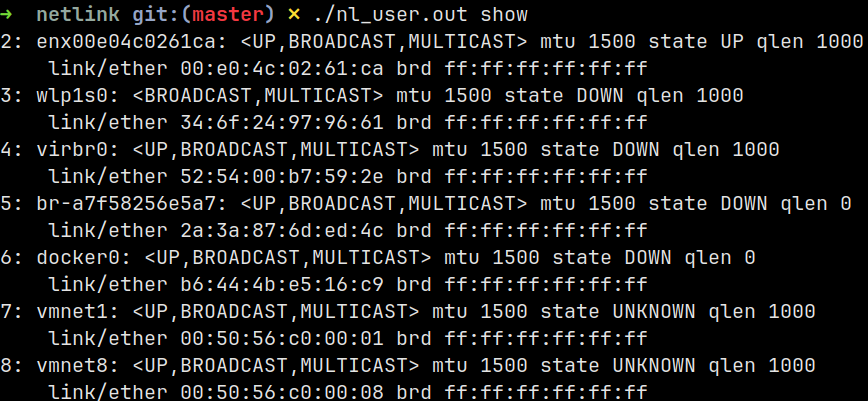
\includegraphics[width=1\textwidth]{./images/show_output.png}
	\caption{Example output of the list of L2 network interfaces}
\end{figure}

Kernel logs after running the command can be inspected by running \texttt{dmesg} with root
privileges:
\begin{lstlisting}[language={Bash}, caption={Showing last kernel logs}]
sudo dmesg 
\end{lstlisting}

Example output of the kernel logs after running the \texttt{./nl\_user.out show} command:
\begin{figure}[ht]
	\centering
	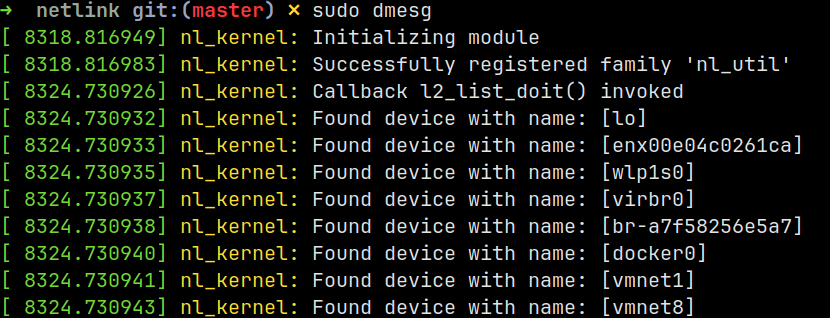
\includegraphics[width=1\textwidth]{./images/dmesg_output.png}
	\caption{Example output of kernel logs after running the \texttt{show} command}
\end{figure}

To display details for a specific interface, the \texttt{./nl\_user.out show <ifindex>}
command is used, where \texttt{ifindex} is the numeric index of the interface.
\begin{lstlisting}[language={Bash}, caption={Displaying interface details}]
./nl_user.out show 2
\end{lstlisting}

Example output from this command:
\begin{figure}[ht]
	\centering
	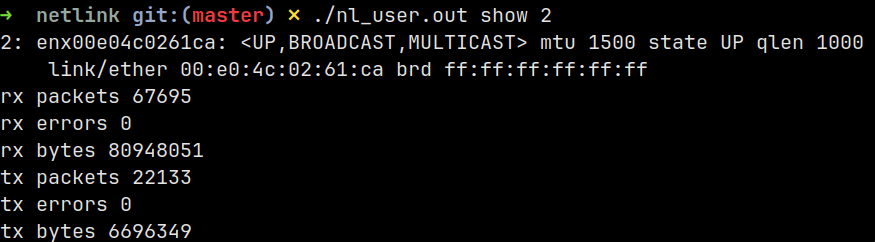
\includegraphics[width=1\textwidth]{./images/show_ifidx_output.png}
	\caption{Example output of detailed information for a specific L2 interface}
\end{figure}

\newpage

\section{Traffic Capture Analysis}
Wireshark has built-in dissectors for well-known Generic Netlink families like
\texttt{nl80211}, which parse commands and attributes based on their definitions (e.g.,
from \texttt{<linux/nl80211.h>}). However, the \texttt{'nl\_util'} family does not have
one, so its payload (commands and attributes) appears as raw hex data.

\begin{figure}[ht]
	\centering
	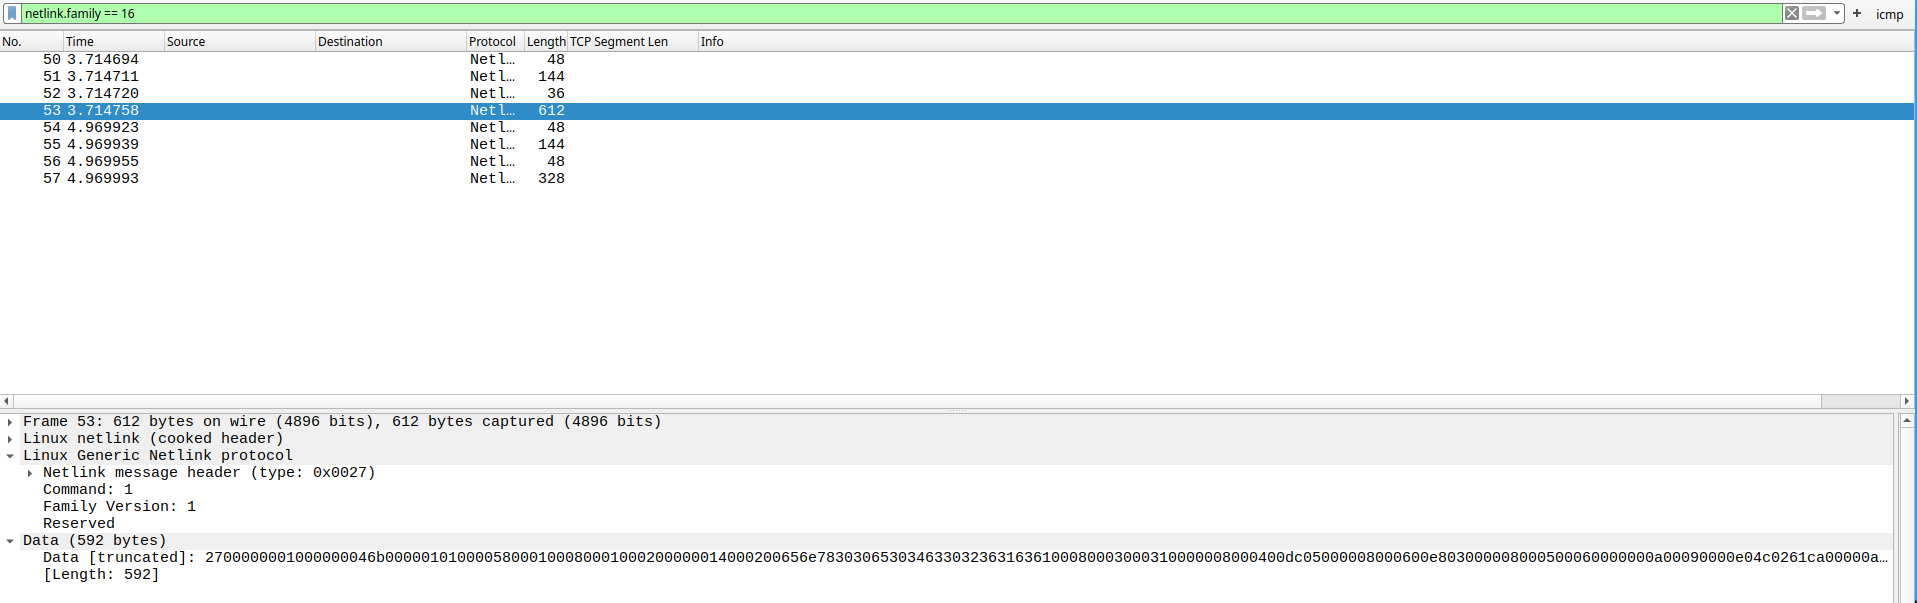
\includegraphics[width=1\textwidth]{./images/raw_hex.png}
	\caption{Netlink capture of the \texttt{./nl\_user.out show} command}
\end{figure}

To identify netlink messages related to the execution of \texttt{ip link show} command,
the underlying system calls are traced using the \texttt{strace} tool. This allows
retrieval of the process ID of the user-space process responsible for sending
requests to the kernel and receiving Layer 2 interface information. The captured Netlink
traffic can then be filtered in Wireshark based on this PID value.

The protocol number used by the \texttt{ip} tool is \texttt{NETLINK\_ROUTE}, which is responsible
for communication between user space and the kernel regarding network configuration. When
\texttt{ip link show} is executed, the kernel responds by dumping information about all
network interfaces. Each interface's information is encapsulated within an
\texttt{rtnetlink} message header.

\begin{figure}[ht]
	\centering
	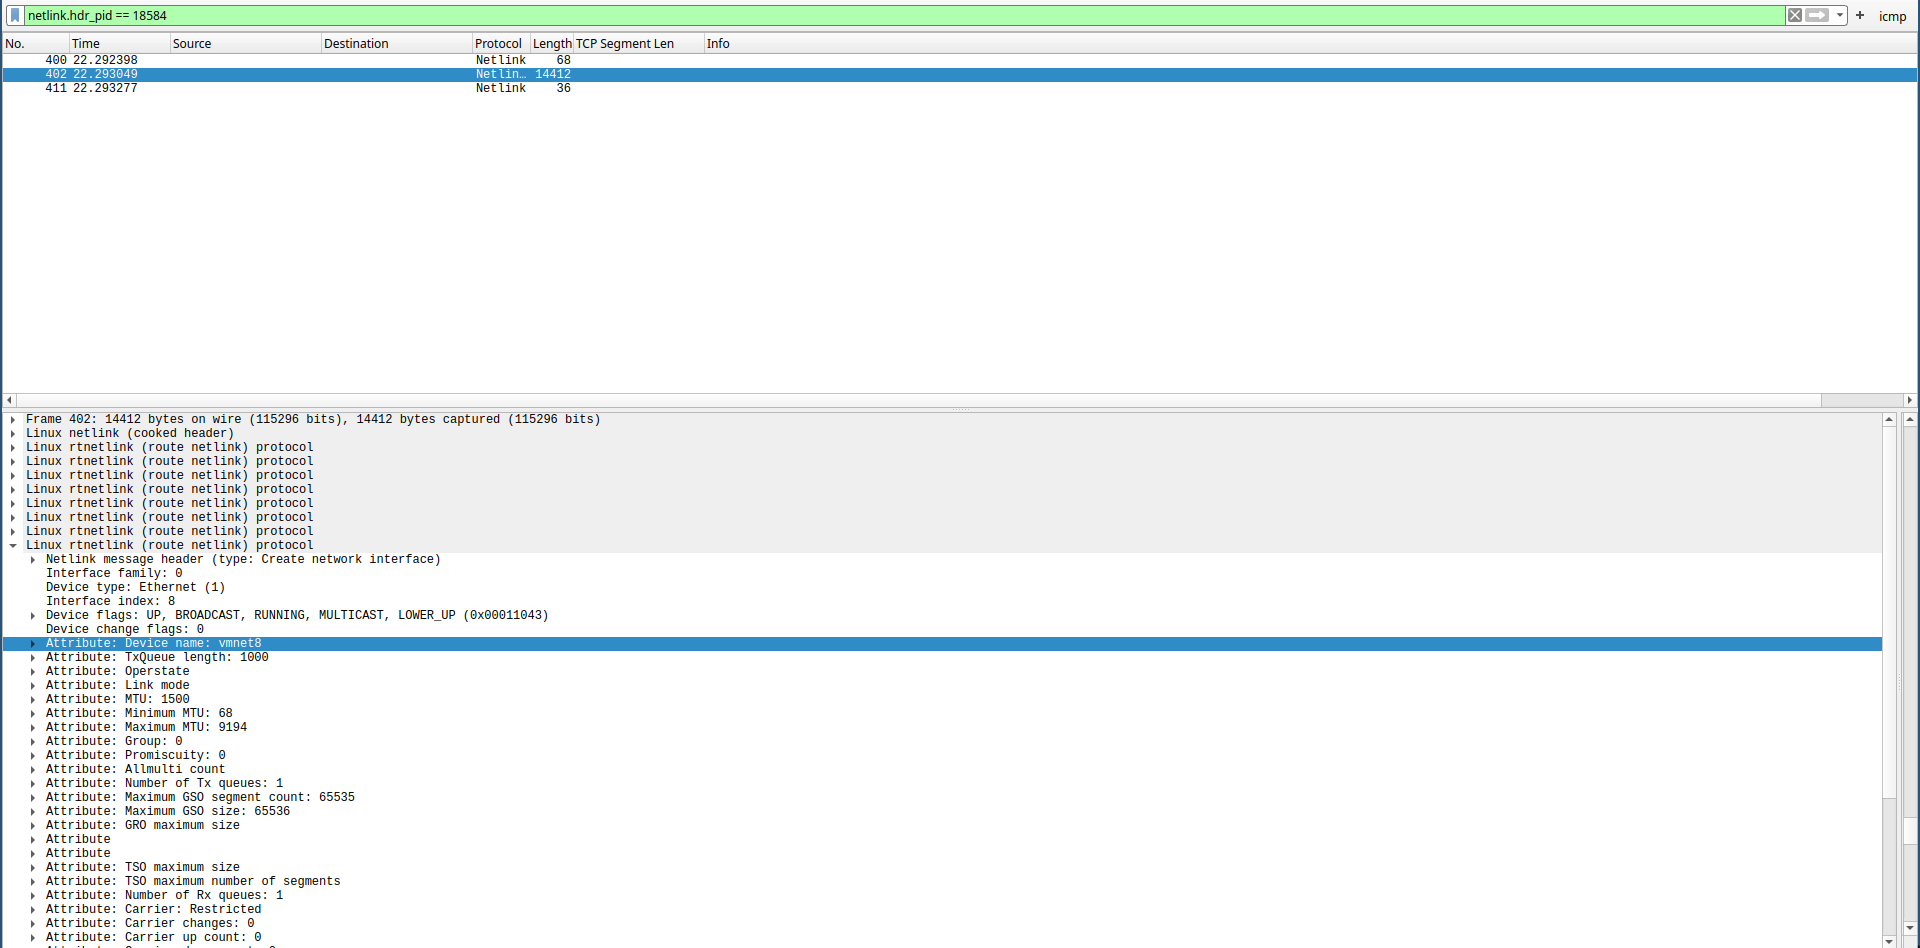
\includegraphics[width=1\textwidth]{./images/ip_link_show_capture.png}
	\caption{Netlink traffic capture of the \texttt{ip link show} command}
\end{figure}

\section{Conclusion}
The implemented Generic Netlink family \texttt{'nl\_util'} supports future extensibility,
allowing additional nested sub-attributes to be added without modifying the top-level
structure. As a part of improvements to be made, the \texttt{l2\_list\_doit} callback
function should ideally perform the same task as the underlying callback function of the
\texttt{ip link show} command does - dumping the information instead of sending it all at once.
However, it is retained as a doit handler for simplicity. Also, it would be beneficial to
implement a dissector for the implemented family.

\section{References}
\begin{itemize}
	\item RFC 3549: Linux Netlink as an IP Services Protocol, \url{https://datatracker.ietf.org/doc/html/rfc3549}
	\item Introduction to Generic Netlink, or How to Talk with the Linux Kernel, \url{https://www.yaroslavps.com/weblog/genl-intro/}
	\item Generic Netlink HOW-TO based on Jamal's original doc \url{https://lwn.net/Articles/208755/}
	\item Introduction to Netlink - Linux Kernel documentation \url{https://docs.kernel.org/userspace-api/netlink/intro.html}
	\item Linux Networking and Network Devices APIs \url{https://docs.kernel.org/networking/kapi.html}
\end{itemize}

\section*{Appendix}
The source code is available on GitHub: \url{https://github.com/sappChak/netdev-genl}

\end{document}
